\subsection{Integrating deduplication, caching, and Docker registries}
\label{sec:design}

%\sysname\ performs file-level deduplication for a Docker registry.
%
\begin{figure*}[t]
	\centering
		%\begin{minipage}{0.225\textwidth}
			\centering
			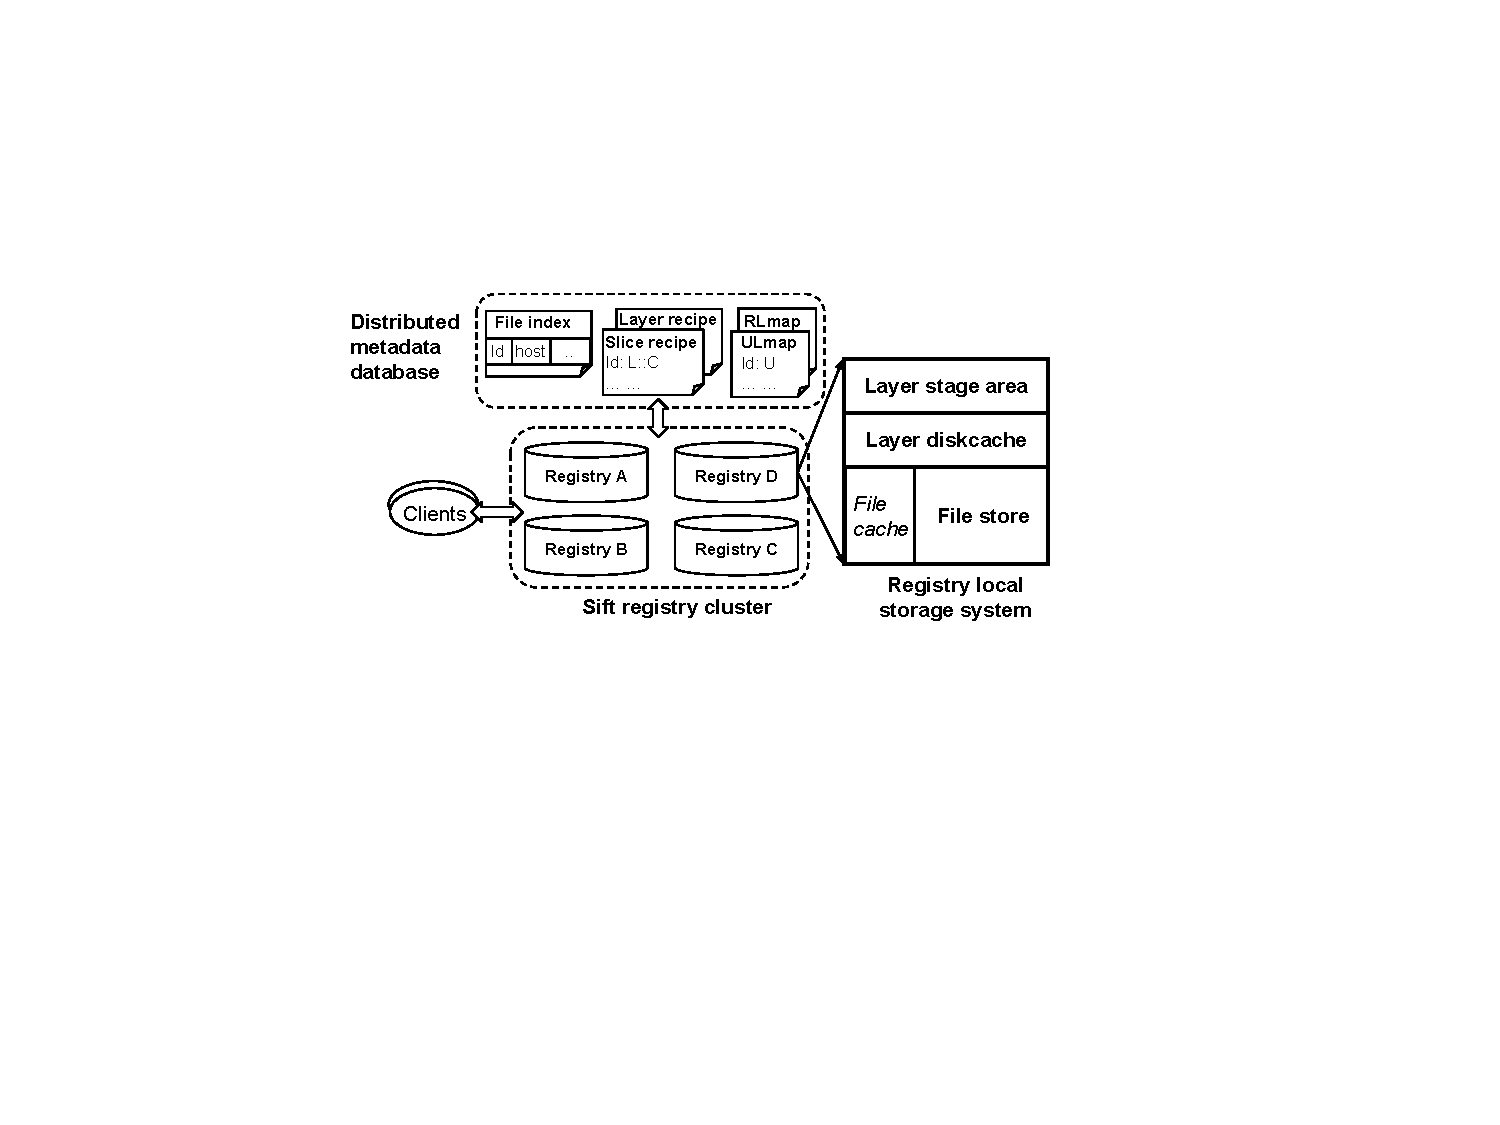
\includegraphics[width=0.9\textwidth]{graphs/sys-architecture.pdf}
%\vspace{-4pt}
			\caption{Architecture of \sysname.}
			%\label{fig:ref_count}
		%\end{minipage}
%	\begin{minipage}{0.225\textwidth}
%		\centering
%		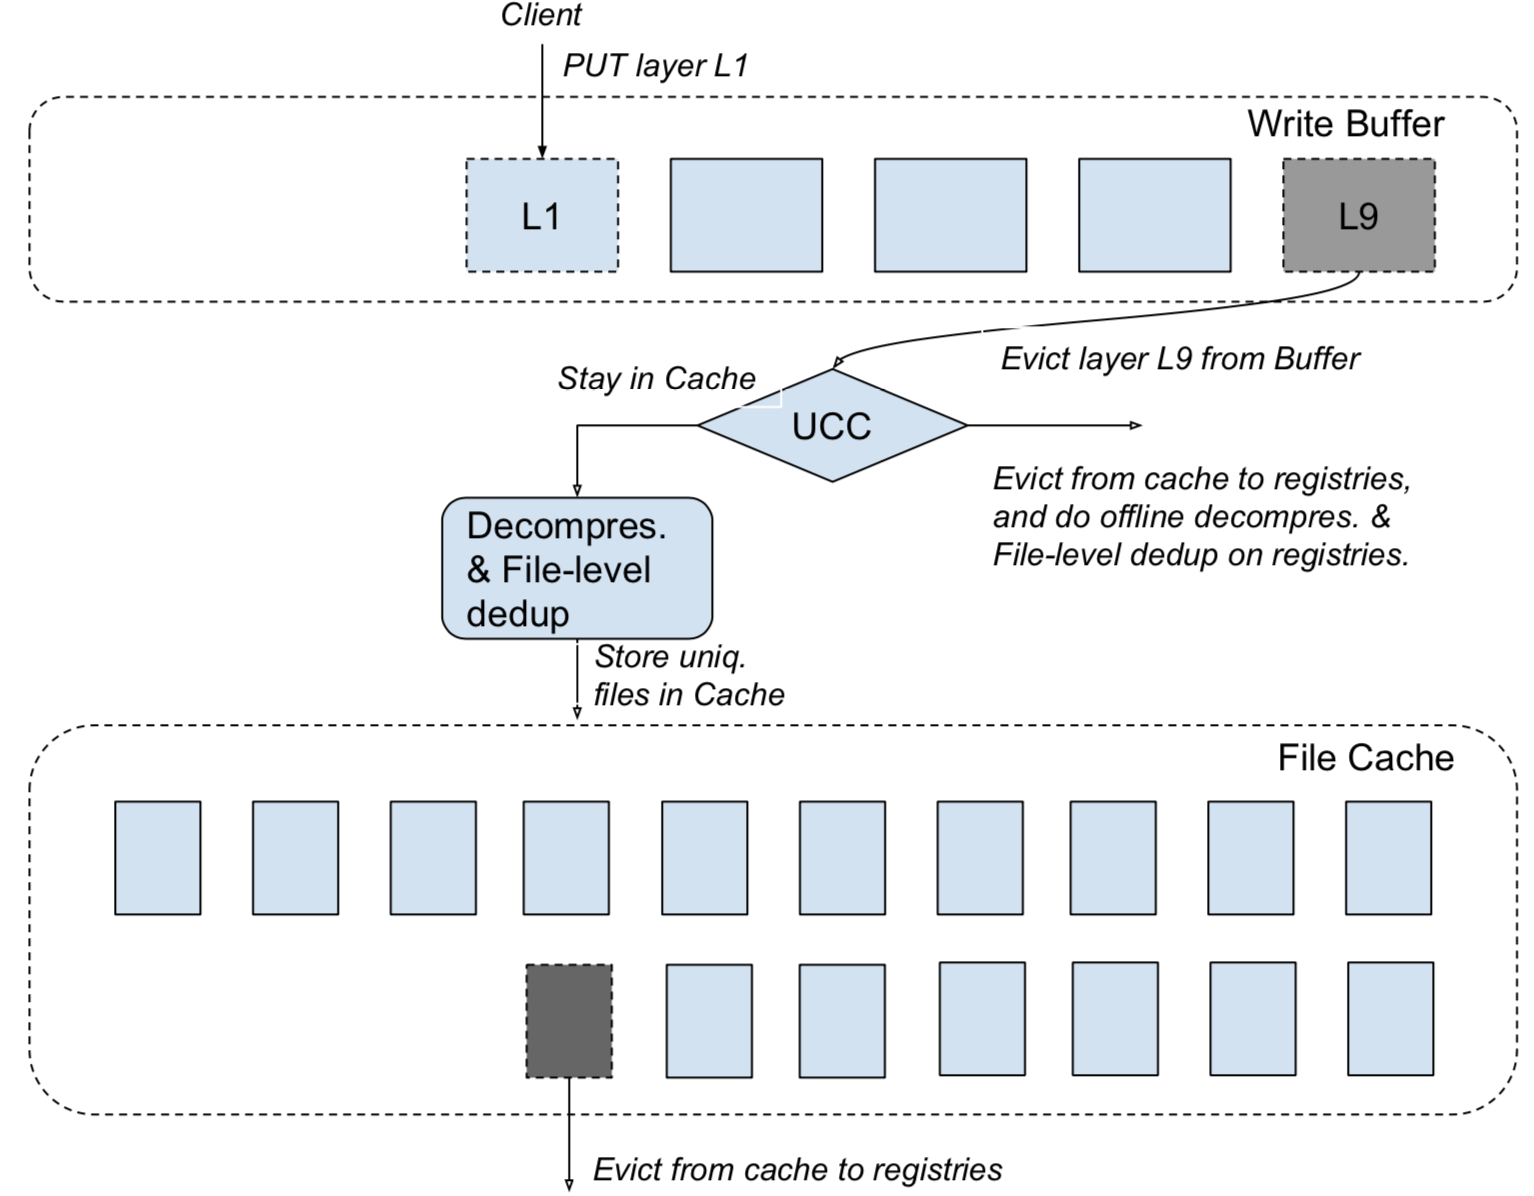
\includegraphics[width=1\textwidth]{graphs/slimmer-cache.png}
%		\caption{CDF of compress. and uncompress. layer size.}
%		\vspace{-3pt}
		\label{fig:sys-overview}
%\vspace{-4pt}
%	\end{minipage}
\end{figure*}

%We designed \sysname\ so that the interface between the Docker clients and the
%registry remains unchanged.
%
%As such, no modifications to the Docker clients are needed.
%
%Below we describe how \sysname\ handles layer pushes and
%pulls at the registry side.
%
%For the sake of this paper, we explain only the main steps omitting smaller
%details.
\Ali{Following text makes no sense.. what are you trying to explain??
\sysname~seamlessly integrates the management of cache, deduplication on
backend storage system (called backend dedup storage), and Docker registries.
Traditionally, caches are placed as close to the requesting client as possible,
such caches are known as proxy caches, or web/HTTP caches for the temporary
storage of frequently requested data to reduce the server's lag.  They are
typically deployed in a regional ISP or within a corporate network.
Deduplication methods are implemented on remote backend storage servers, and
transparently remove duplicates from the incoming data stream and restore the
data for read requests.}

\Ali{Following information should be part of Background section..
Docker registry is a web server that serves Docker
\texttt{pull} and Docker \texttt{push} requests.  Although Docker registry is a
layer-level content addressable storage system holding all the images, it
delegates storage to drivers which interact with either a local file system or
a remote cloud storage like S3, Microsoft Azure, OpenStack Swift, and Aliyun
OSS.  Intuitively, registries can be deployed as a proxy cache to host
frequently requested layers.  This approach, a registry as a pull-through
cache, speeds up image pulls and improves overall performance.  At the same
time, the backend cloud storage can leverage deduplication to save storage
space.}


\subsection{Design challenges}
There are several unique problems concerning the integration
of caching and deduplication to the Docker registry.
%
First, for caching layers, \texttt{pull} layer requests are difficult to
predict because same layers are not accessed frequently.
We observed that, on average, around half of the cached layers' are not
accessed again for at least 4 hours which means that if we
cache a layer, we might need to wait hours to get a hit on that layer.  
This is
because when a user pulls an image from the registry, the Docker daemon on the
requesting host will only pull the layers that are not locally stored.
\Ali{I do not understand the following sentence.}
Moreover, we have to consider that a user might deploy an applications on
multiple machines, so it's not easy to predict when a user will access which layers. 
Ali Anwar et
al., proposed a prefetching method~\cite{dockerworkload} based on the
\texttt{push}-\texttt{pull} relationship: when there is a \texttt{PUSH} layer
request directly followed by a \texttt{GET} manifest request, a \texttt{GET}
layer request will most probably follow. 
However, based on our trace\HA{we have to mention which trace???} analysis,
only half of the \texttt{pull} layer
requests have a precedent \texttt{PUSH} layer request within the trace
collecting duration of 75 days. This means that, after a user pushes a layer
to the registry, it takes a few days, weeks, or even months for a user to make
a \texttt{pull} request.
\Ali{The above statement is incorrect. You have to distinguish between GET layer requests
that are issued after a (PUSH layer + GET manifest) request and a normal GET layer request.
FAST paper only talk about case 1. Whereas you are generalizing that any GET layer request
should have a precedent GET layer request which is wrong. We can make a case
that not all GET layers requests have a precedent PUSH layer request but we can
not say that it takes a few days, weeks, or even months for a user to make a pull
layer request after a push layer request.}

Second, we can not deduplicate compressed layers. Hence, for deduplication each layer
needs to be uncompressed and then undergo a file-level deduplication. Similarly,
to restore a layer, we need to fetch files from multiple servers and then compress
them in to a tar file. 
This whole process can cause a 
considerable overhead on \texttt{pull} layer requests performance.
\Ali{Explain how push layer requests are not effected?}


\subsection{Design}
To meet these challenges, we propose a new registry design featuring a user
behavior based cache to reduce the performance degradation caused by
deduplication on backend storage system (Figure~\ref{fig:sys-overview}).  Based
on our observation, user's active time is easier to predict as shown in
Figure~\ref{fig:reusetime}. Our cache design considers user
behavior such as when a user is most likely to be active for
layer evictions from the cache.

Considering that layer size is around several megabyte on
average~\cite{dockerworkload}, a small main memory cache cannot accommodate
many active users' layers. To address this issue, we couple main memory and
flash memory to provide separate caching for layers and \emph{deduped} files.
We call compressed layer cache cache and \emph{deduped} files cache,
\emph{layer buffer} and \emph{file cache}, respectively.
For handling
cache evictions, we first evict inactive users' layers from the layer buffer.
Next, we \emph{dedup} the evicted layers, then store the \emph{deduped} files
into the file cache (detailed in \cref{sec:design_operations}). 
%the following operations: decompressing each evicted layer and comparing its
%containing files with the files that are already stored in the file cache,
%eliminating duplicate files, that is, only storing the unique files on flash
%storage.
When a user requests a
layer not present in the layer buffer, the request is forwarded to the
file cache (detailed in~\cref{sec:design_operations}). 
If a layer is not found in both the layer buffer and the
file cache, the request is forwarded to the backend dedup storage system.
Note that during layer deduplication, uncompressed layer files are
scattered across multiple servers.
We call all the files belonging to a layer on a specific server a
\emph{slice} of the layer.
All the slices for a layer are fetched in parallel for performance improvement.
%
%To avoid the network latency caused by fetching slices from different servers and
%assembling them into a whole compressed layer, the \texttt{pull} request will
%be separately forwarded to all the backend servers that store the requested
%layer's slice.  
%
Each backend server compresses the slice and directly send the compressed slices back to the user.
We modify the Docker client
interface such that when it receives all the compressed slices, it can
decompress them into a single layer. 
Furthermore, compressing slices
of layers in parallel considerably mitigates the compression latency caused by
compressing a whole layer since compression time depends on the size of the
uncompressed data.
%to cache layers and cache unique files after decompression and deduplication,
%respectively.  consists of a \emph{layer buffer} and a \emph{file cache}.  The
%layer buffer stores all the newly pushed layers in memory.  Although accessing
%memory is very fast, the size of main memory is limited. 




 
